%; whizzy chapter
% -initex iniptex -latex platex -format platex -bibtex jbibtex -fmt fmt
% $B0J>e(B whizzytex $B$r;HMQ$9$k>l9g$N@_Dj!#(B

%     Kansai Debian Meeting resources
%     Copyright (C) 2007 Takaya Yamashita
%     Thank you for Tokyo Debian Meeting resources

%     This program is free software; you can redistribute it and/or modify
%     it under the terms of the GNU General Public License as published by
%     the Free Software Foundation; either version 2 of the License, or
%     (at your option) any later version.

%     This program is distributed in the hope that it will be useful,
%     but WITHOUT ANY WARRANTY; without even the implied warranty of
%     MERCHANTABILITY or FITNESS FOR A PARTICULAR PURPOSE.  See the
%     GNU General Public License for more details.

%     You should have received a copy of the GNU General Public License
%     along with this program; if not, write to the Free Software
%     Foundation, Inc., 51 Franklin St, Fifth Floor, Boston, MA  02110-1301 USA

%  preview (shell-command (concat "evince " (replace-regexp-in-string "tex$" "pdf"(buffer-file-name)) "&"))
% $B2hA|%U%!%$%k$r=hM}$9$k$?$a$K$O(Bebb$B$rMxMQ$7$F(Bboundingbox$B$r:n@.!#(B
%(shell-command "cd image200708; ebb *.png")

%%$B$3$3$+$i%X%C%@3+;O!#(B

\documentclass[mingoth,a4paper]{jsarticle}
\usepackage{kansaimonthlyreport}
\usepackage[dvips]{xy}

% $BF|IU$rDj5A$9$k!"Kh7nJQ$o$j$^$9!#(B
\newcommand{\debmtgyear}{2009}
\newcommand{\debmtgdate}{27}
\newcommand{\debmtgmonth}{09}
\newcommand{\debmtgnumber}{27}

\begin{document}

\begin{titlepage}

% $BKh7nJQ99$9$kItJ,!"K\J8$NKvHx$b=$@5$9$k$3$H$r$o$9$l$:$K(B

 $BBh(B\debmtgnumber{}$B2s(B $B4X@>(B Debian $BJY6/2q;qNA(B

\vspace{2cm}

\begin{center}

\includegraphics{image200802/kansaidebianlogo.png}
\end{center}

\begin{flushright}
\hfill{}$B4X@>(B Debian $BJY6/2qC4Ev<T(B $B$N$,$?!&ARI_!&:4!9LZ(B\\
\hfill{}\debmtgyear{}$BG/(B\debmtgmonth{}$B7n(B\debmtgdate{}$BF|(B
\end{flushright}

\thispagestyle{empty}
\end{titlepage}

\dancersection{Introduction}{Debian JP}
 
 $B4X@>(B Debian $BJY6/2q$O(BDebian GNU/Linux $B$N$5$^$6(B
 $B$^$J%H%T%C%/(B($B?7$7$$%Q%C%1!<%8!"(BDebian $BFCM-$N5!G=$N;EAH!"(BDebian $B3&7($G5/(B
 $B$3$C$?=PMh;v!"$J$I$J$I!K$K$D$$$FOC$79g$&2q$G$9!#(B

 $BL\E*$H$7$F<!$N;0$D$r9M$($F$$$^$9!#(B
 \begin{itemize}
  \item ML$B$d7G<(HD$G$O$J$/!"D>@\4i$r9g$o$;$k;v$G$N>pJs8r49$NB%?J(B
  \item $BDj4|E*$K=8$^$l$k>l=j(B
  \item $B;qNA$N:n@.(B
 \end{itemize}

 $B$=$l$G$O!"3Z$7$$0l;~$r$*3Z$7$_2<$5$$!#(B

\newpage

\begin{minipage}[b]{0.2\hsize}
 {\rotatebox{90}{\fontsize{80}{80}
{\gt $B4X@>%G%S%"%sJY6/2q(B}}}
\end{minipage}
\begin{minipage}[b]{0.8\hsize}
\hrule
\vspace{2mm}
\hrule
\setcounter{tocdepth}{1}
\tableofcontents
\vspace{2mm}
\hrule
\end{minipage}

\dancersection{$B:G6a$N(BDebian$B4X78$N%$%Y%s%HJs9p(B}{}

%-------------------------------
\dancersection{GUI$B$,$D$$$F3J9%NI$/$J$C$?(Breportbug$B$r;H$C$F$_$h$&(B}{$B$N$,$?$8$e$s(B}

\subsection{$B$O$8$a$K(B}

Debian$B$N%P%0Js9p;Y1g%D!<%k(Breportbug$B$,!"%P!<%8%g%s(B3.99.0$B$+$i(BGTK2$B$rMxMQ$7$?(B
$B%f!<%6!<%$%s%?!<%U%'!<%9$,;H$($k$h$&$K$J$C$F$$$^$7$?$,!"$"$^$jCN$i$l$F$$$J$$(B
$B$N$G(Breportbug$B$N;H$$J}$b7s$M$F=q$$$F$_$^$7$?!#(B

\subsubsection{$B$*$o$S(B}

$B!V;H$C$F$_$h$&!W$H%?%$%H%k$K=q$-$^$7$?$,!"<B:]$K(BGTK2$B%$%s%?!<%U%'!<%9$G;H(B
$B$&$H(Bquerybts$B$,$&$^$/F0$+$:EPO?$5$l$?%P%0$rI=<($9$k$3$H$,$G$-$J$+$C$?$j!"(B
$BLa$k%\%?%s$GLa$k$HF~NO$,$G$-$J$+$C$?$j$HIT6q9g$"$j$^$9!#$G$9$N$G!V;H$&!W(B
$B$K$OFq$7$$$H$3$m$b$"$j$^$9$,!"$H$j$"$($:$3$s$J46$8$H$$$&$3$H$rCN$C$F$b$i(B
$B$($l$P;W$$$^$9!#(B

\subsection{reportbug$B$H$O(B}

Debian$B$r;H$C$F$$$FH/8+$7$?%P%0$O!"7h$a$i$l$?=q<0$K$7$?$,$C$F=q$$$?%a!<%k(B
$B$r(BDebian$B$N%P%0DI@W%7%9%F%`(B(Bug Tracking System.$BDL>N(BBTS)$B$KAw$k$3$H$K$h$C$F(B
$B%P%0$rJs9p$9$k$3$H$,$G$-$^$9(B \footnote{$B%P%0%l%]!<%H$+$i;22C$9$k(BDebian$B%Q%C(B
$B%1!<%83+H/(B / $BLZ2<(B $BC#Li(B ($B$"$s$I$-$e$a$s$F$C$I(B $B$G$S$"$s(B 2008$BG/2F9f(B)

\url{http://tokyodebian.alioth.debian.org/pdf/debianmeetingresume2008-natsu.pdf}}$B!#$G$9$,%P%0Js9p$K47$l$F$$$J$$$H!"7h$a$i$l$?(B
$B=q<0$G%a!<%k$r=q$/$3$H$O$b$A$m$s$N$3$H!"%P%0=$@5$KI,MW$J%Q%C%1!<%8>pJs$J(B
$B$I$r1L$l$J$/=8$a$?$j$9$k$3$H$OBgJQ$J$3$H$G$9!#(B

reportbug$B$O!"$=$&$$$C$?%P%0Js9p$NIiC4$r8:$i$9$?$a$N%D!<%k$G!"%P%08!:w$+$i!"(B
$B%P%0Js9p$N$?$a$N%Q%C%1!<%8>pJs$N<}=8!"%P%0EPO?$KI,MW$J%a!<%k$N=q<0@07A!"(B
$BJs9p%a!<%k$NAw?.$^$G9T$C$F$/$l$k%D!<%k$G$9!#(B

\subsection{reportbug$B$N%$%s%9%H!<%k(B}

Debian$B%$%s%9%H!<%k;~$K!VI8=`%7%9%F%`!W$rA*Br$9$k$H!"(Breportbug$B$O%$%s%9%H!<(B
$B%k$5$l$^$9$,!"(BGTK2$B$dC<Kv>e$G$N%a%K%e!<%$%s%?!<%U%'!<%9$KI,MW$J(BRecommends
$B$d(BSuggests$B%Q%C%1!<%8$O%$%s%9%H!<%k$5$l$J$$$N$G!"2~$a$F(Breportbug$B$r%$%s%9%H!<(B
$B%k$7$^$9!#(B

\begin{commandline}
 # apt-get update
 # apt-get remove reportbug
 # apt-get -o APT::Install-Suggests=true --install-recommends -y install reportbug
\end{commandline}

$B$^$I$m$C$3$7$$$3$H$r$7$F$$$^$9$,!"$9$G$K%$%s%9%H!<%k$5$l$?%Q%C%1!<%8$N(B
Recommends$B$d(BSuggests$B%Q%C%1!<%8$r%9%^!<%H$K%$%s%9%H!<%k$9$k$K$O$I$&$7$?$i(B
$B$$$s$G$7$g$&$+(B?

\subsection{reportbug$B$r5/F0(B}

reportbug$B$r5/F0$7$^$9!#(B

$B%G%9%/%H%C%W$N%a%K%e!<(B([$B%"%W%j%1!<%7%g%s(B]$B"*(B[$B%7%9%F%`%a(B
$B%K%e!<(B]$B"*(B[reportbug])$B$+$i5/F0$9$k$H!"(BGTK2$B%$%s%?!<%U%'!<%9$N%&%#%s%I%&$,3+(B
$B$-$^$9!#C<Kv$+$i5/F0$9$k$H%a%C%;!<%8$,I=<($5$l$^$9!#(B

\begin{commandline}
 $ reportbug 
\end{commandline}

\begin{figure}[h]
 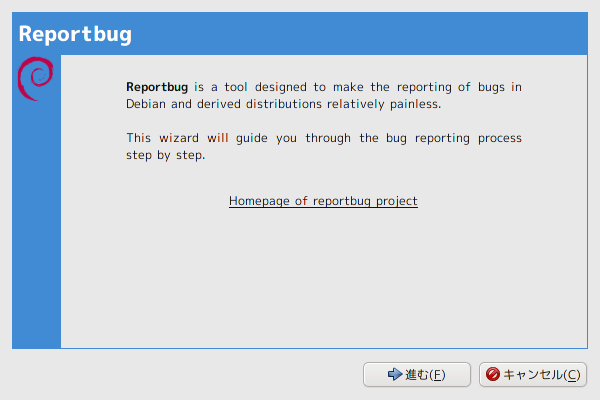
\includegraphics[scale=0.5]{image200909/reportbug-initial.png}
 \caption[reportbug$B$N(BGTK2$B%$%s%?!<%U%'!<%9(B]{reportbug$B$N(BGTK2$B%$%s%?!<%U%'!<%9(B}
\end{figure}

\subsection{$B=i4|@_Dj(B}
reportbug$B$r=i$a$F5/F0$9$k$H!"(Breportbug$B$r;H$&$?$a$N@_Dj$r?R$M$i$l$^$9!#(B
$B=i4|@_Dj$NESCf!"%P%0Js9p%a!<%k$rAw?.$9$k$?$a$N%a!<%k4D6-$K$D$$$F?R$M$i$l(B
$B$k$N$G!"$"$i$+$8$a%a!<%k$N@_Dj$r3NG'$7$F$*$$$F$/$@$5$$!#(B
$B@_DjNc$G$O!"(BGmail$B$r;H$C$F$$$k$3$H$rA0Ds$KOC$r?J$a$^$9!#(B

\begin{itemize}
 \item $B;29M(B: $B$=$NB>$N%a!<%k(B $B%/%i%$%"%s%H$N@_Dj(B - Gmail $B%X%k%W(B:

\url{http://mail.google.com/support/bin/answer.py?hl=jp&answer=13287}
\end{itemize}

\begin{commandline}
Welcome to reportbug! Since it looks like this is the first time you have used reportbug, we are configuring its behavior.

These settings will be saved to the file "/home/hoge/.reportbugrc", which you will be free to edit further.                
Please choose the default operating mode for reportbug.                                                                   

1 novice    Offer simple prompts, bypassing technical questions.

2 standard  Offer more extensive prompts, including asking about things that a moderately sophisticated user would be
            expected to know about Debian.                                                                           

3 advanced  Like standard, but assumes you know a bit more about Debian, including "incoming".

4 expert    Bypass most handholding measures and preliminary triage routines. This mode should not be used by people
            unfamiliar with Debian's policies and operating procedures.                                             

Select mode: [novice] 
\end{commandline}

$B%&%'%k%+%`%a%C%;!<%8$H@_Dj$O(B~/.reportbugrc$B$KJ]B8$5$l$F$$$^$9$HFs$D$N$*CN(B
$B$i$;$N8e!"(Breportbug$B$G;H$&%b!<%I$K$D$$$F?R$M$F$$$^$9!#$H$j$"$($:$O:Y$+$$$3(B
$B$H$h$j%P%0Js9p$@$1$K9J$j$?$$$N$G!"(Bnovice$B$N$^$^$G$h$$$G$7$g$&!#(B

\newpage

\begin{commandline}
Please choose the default interface for reportbug.

1 text   A text-oriented console user interface

2 gtk2   A graphical (GTK+) user interface.

3 urwid  A menu-based console user interface

Select interface: 2
\end{commandline}

$B$I$N%f!<%6!<%$%s%?!<%U%'!<%9$r;H$&$+A*Br$7$^$9!#(B
$B:#2s$O%F!<%^$K$=$C$F(Bgtk2$B$rA*$S$^$7$?!#<B:]$K;H$&$H$J$k$H(Burwid$B$,;H$$$d$9(B
$B$$$H;W$$$^$9!#(B

\begin{commandline}
Will reportbug often have direct Internet access? (You should answer yes to this question unless you know what you are doing
and plan to check whether duplicate reports have been filed via some other channel.) [Y|n|q|?]?
\end{commandline}

$B%$%s%?!<%M%C%H$K@\B3$7$F$$$k$+$G$9$,!"$*$=$i$/$[$H$s$I$N?M$O@\B3$7$F$$$k(B
$B$H;W$&$N$G!"(By$B$HEz$($^$9!#(B

\begin{commandline}
What real name should be used for sending bug reports?
[Hogewo HOGETA]>
\end{commandline}

$B%P%0Js9p$K;H$&L>A0$r@_Dj$7$^$9!#(B

\begin{commandline}
Which of your email addresses should be used when sending bug reports? (Note that this address will be visible in the bug
tracking system, so you may want to use a webmail address or another address with good spam filtering capabilities.)
[example@gmail.com]>
\end{commandline}

$B%P%0Js9p$K;H$&%a!<%k%"%I%l%9$r@_Dj$7$^$9!#(B
$B$3$3$G5$$r$D$1$J$$$H$$$1$J$$$3$H$O!"$3$3$G@_Dj$7$?%a!<%k%"%I%l%9$O%P%0Js(B
$B9p$r$9$k$H8x3+$5$l$^$9!#$"$^$j8x3+$7$?$/$J$$%a!<%k%"%I%l%9$O@_Dj$7$J$$$[(B
$B$&$,$h$$$G$7$g$&!#(B

\begin{commandline}
Do you have a "mail transport agent" (MTA) like Exim, Postfix or SSMTP configured on this computer to send mail to the
Internet? [Y|n|q|?]? n
\end{commandline}

$B%P%0Js9p$r$9$k%^%7%s$G%a!<%k%5!<%P!<$,F0$$$F$$$k$+?R$M$F$$$^$9!#(B
Gmail$B$N(BSMTP$B%5!<%P!<$r;H$C$FAw?.$9$k$N$G!"$3$3$G$O(Bn$B$HEz$($^$9!#(B

\begin{commandline}
Please enter the name of your SMTP host.  Usually it's called something
 like "mail.example.org" or "smtp.example.org".
If you need to use a different port than default, use the <host>:<port> alternative format.

Just press ENTER if you don't have one or don't know.
> smtp.gmail.com:587
\end{commandline}

$BAw?.$9$k(BSMTP$B%5!<%P!<$rEPO?$7$^$9!#(B
Gmail$B$N(BSMTP$B%5!<%P!<$N%"%I%l%9$O(Bsmtp.gmail.com$B!"%]!<%HHV9f$O(B587$B$J$N$G!"(B
smtp.gmail.com:587$B$HEPO?$7$^$9!#(B

\begin{commandline}
If you need to use a user name to send email via "smtp.gmail.com:587" on your computer, please enter that user name. Just
press ENTER if you don't need a user name.
> nogajun@gmail.com
\end{commandline}

SMTP$B%5!<%P!<$rMxMQ$9$k$?$a$N%f!<%6!<L>$rEPO?$7$^$9!#(B
Gmail$B$N(BSMTP$B%5!<%P!<$r;H$&$K$O%I%a%$%sL>$b4^$a$?%f!<%6!<L>$,I,MW$J$N$G!"(B<$B%f!<%6!<(B
$BL>(B>@gmail.com$B$HEPO?$7$^$9!#(B

\begin{commandline}
Does your SMTP host require TLS authentication? [y|N|q|?]? y
\end{commandline}

SMTP$B$O(BTLS$B$r;H$&$+$NLd$$$K$D$$$F$O!"(BGmail$B$G$OI,MW$J$N$G(By$B$HEz$($^$9!#(B

\begin{commandline}
Please enter the name of your proxy server. It should only use this parameter if you are behind a firewall. The PROXY
argument should be formatted as a valid HTTP URL, including (if necessary) a port number; for example,
http://192.168.1.1:3128/. Just press ENTER if you don't have one or don't know.
>
\end{commandline}
Proxy$B$K$D$$$F?R$M$F$$$^$9!#;H$C$F$$$l$P@_Dj$7$^$9!#;H$C$F$$$J$1$l$P6u$N$^$^(B
$B$G(BEnter$B%-!<$r2!$7$^$9!#(B

\begin{commandline}
Default preferences file written. To reconfigure, re-run reportbug with the "--configure" option.
\end{commandline}
$B=i4|@_Dj$,=*$o$j$^$7$?!#$b$&0lEY!"@_Dj$r$d$jD>$7$?$$$H$-$O!"(B--configure$B%*(B
$B%W%7%g%s$r$D$1$F5/F0$9$k$H$d$jD>$9$3$H$,$G$-$^$9!#(B

\subsection{reportbug$B$r;H$C$F$_$k(B}

 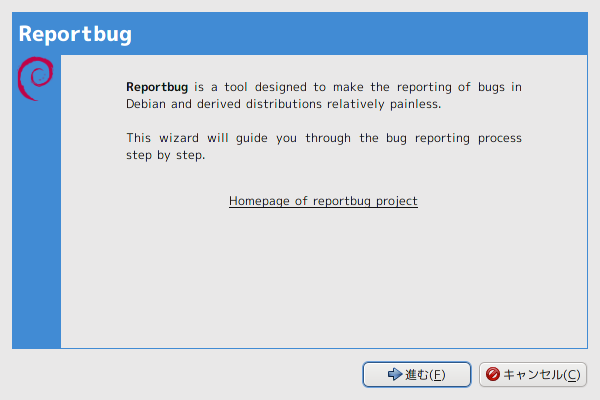
\includegraphics[scale=0.5]{image200909/reportbug-1.png}

$B5/F0$9$k$H$3$s$J46$8$G$9!#%&%#%6!<%I7A<0$J$N$G$o$+$j$d$9$$$H;W$$$^$9!#(B

 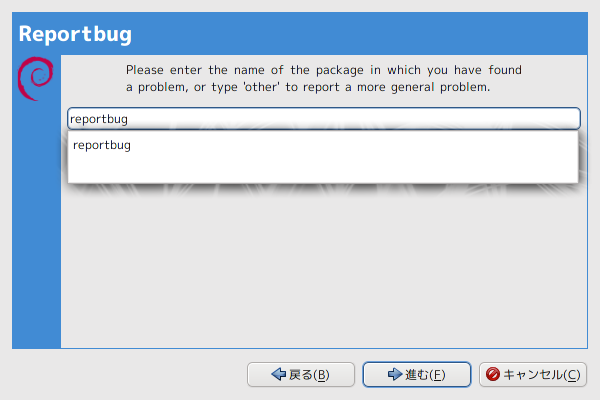
\includegraphics[scale=0.5]{image200909/reportbug-2.png}

$B%P%0$r8+$D$1$?%Q%C%1!<%8L>$rF~NO$7$^$9!#%Q%C%1!<%8L>$NF,$r2?J8;z$+F~NO$9(B
$B$k$H!"%$%s%9%H!<%k$5$l$F$$$k%Q%C%1!<%8$N8uJd$rI=<($7$F$/$l$^$9!#(B

 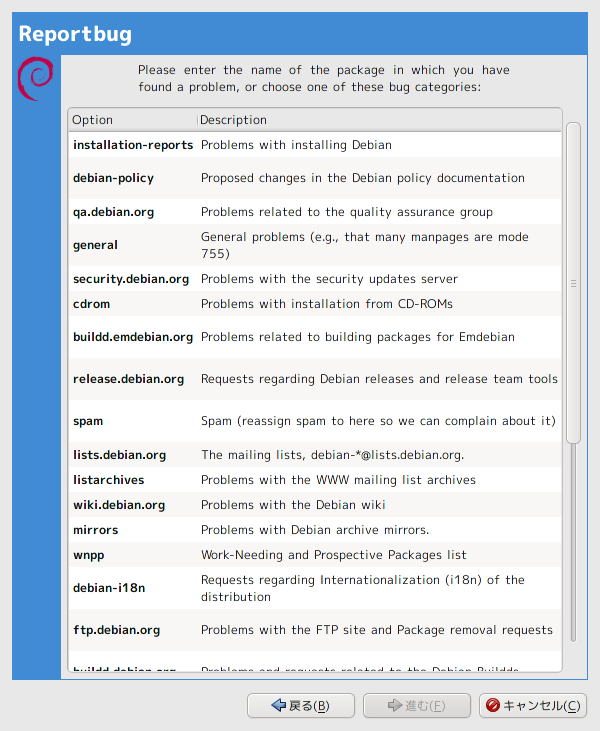
\includegraphics[scale=0.5]{image200909/reportbug-8.png}

$B%Q%C%1!<%8L>$NF~NO$G(Bother$B$HF~NO$9$k$H$3$N2hLL$K$J$j$^$9!#$3$l$O5<;w%Q%C%1!<(B
$B%8$N0lMw$G$9!#%Q%C%1!<%80J30$K8+$D$1$?(BDebian$B$K4XO"$9$kLdBj$r5<;w%Q%C%1!<(B
$B%8$N%P%0$H$7$FEPO?$7$^$9!#(B

\begin{itemize}
 \item Debian -- Debian $B%P%0DI@W%7%9%F%`(B - $B5<;w%Q%C%1!<%8(B:

\url{http://www.debian.org/Bugs/pseudo-packages.ja.html}

\end{itemize}

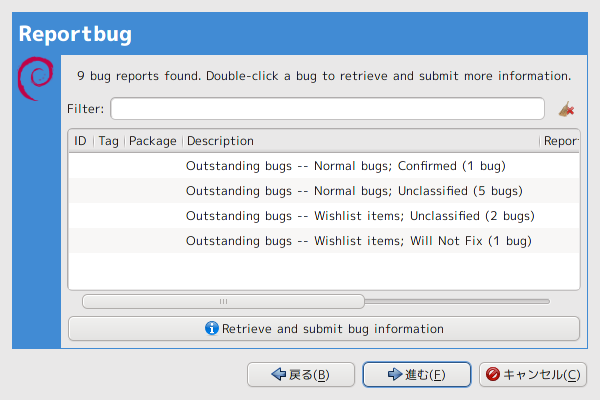
\includegraphics[scale=0.5]{image200909/reportbug-3.png}

$BK\Mh$J$i$P$3$3$KEPO?$5$l$?%P%0$,I=<($5$l$F!":#$+$iEPO?$7$h$&$H$7$?%P%0$,(B
$B$9$G$KEPO?:Q$_$+$I$&$+3NG'$G$-$k$N$G$9$,!"(BGTK2$B%$%s%?!<%U%'!<%9$@$H(B
querybts$B$,$&$^$/F0$+$J$/$F(B(\#432178)$B!"%@%V%k%/%j%C%/$r$7$F$b2?$bI=<($5$l(B
$B$^$;$s!#;DG0!#(B

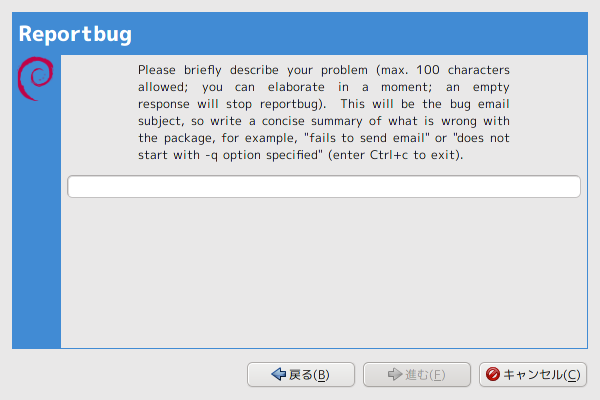
\includegraphics[scale=0.5]{image200909/reportbug-4.png}

$B%P%0$,$^$@EPO?$5$l$F$$$J$+$C$?$H$7$F<!$K?J$`$H!"%P%0$rEPO?$9$k2hLL$KF~$j(B
$B$^$9!#$3$3$G$O%P%0$N35MW$r4J7i$K=q$-$^$9!#(B

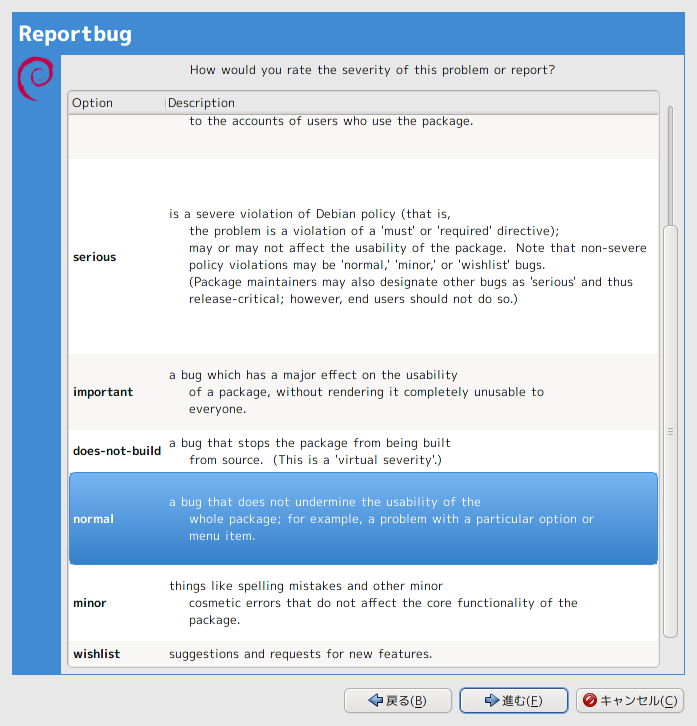
\includegraphics[scale=0.5]{image200909/reportbug-5.png}

$B%P%0$N<oN`$r;XDj$7$^$9!#<oN`$O(BCritical$B$d(BSerious$B$N$h$&$J?<9o$J$b$N$+$i!"Ds(B
$B0F$N(BWhishlist$B$^$G$"$j$^$9!#DL>o$O(Bnormal$B$G$$$$$H;W$$$^$9!#(B

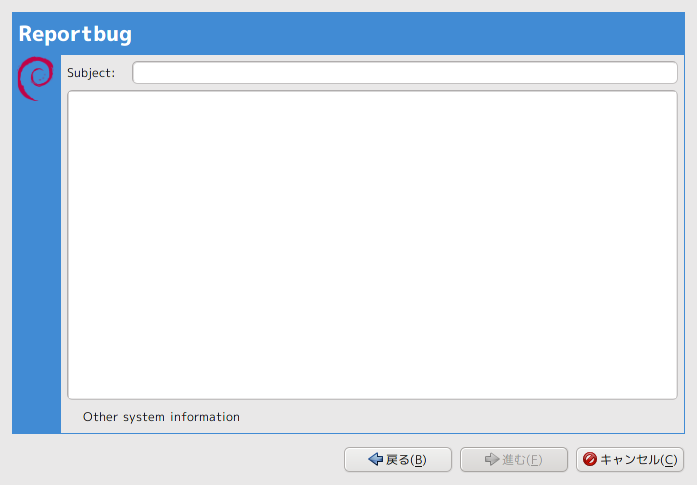
\includegraphics[scale=0.5]{image200909/reportbug-6.png}

$B$3$3$G$O!"%P%0$NFbMF$r=q$-$^$9!#(B
$B%9%/%j!<%s%7%g%C%H$N$?$a$KE,Ev$J$3$H$r=q$$$F;#$C$F$$$?$N$G(BSubject$B$O>C$7$F(B
$B$$$^$9$,!"DL>o$O(BSubject$B$N2U=j$K>e$G=q$$$?%P%0$N35MW$,F~$C$F$$$^$9!#(B

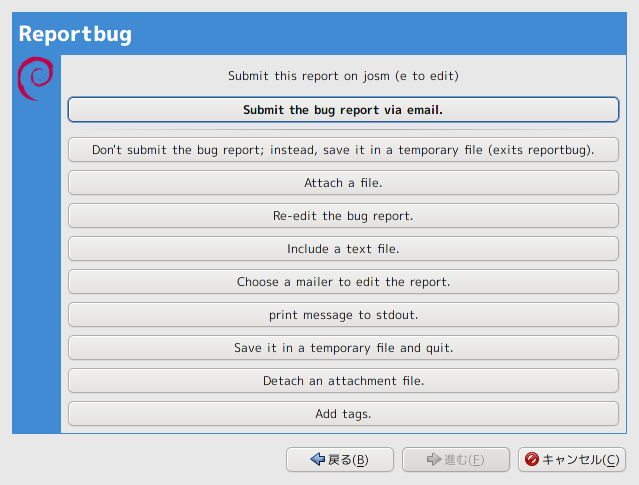
\includegraphics[scale=0.5]{image200909/reportbug-7.png}

$B%P%0$NFbMF$r=q$-=*$o$C$F?J$`$H!"$3$N2hLL$K$J$j$^$9!#(B

$B$3$N;~E@$G$O$^$@%a!<%k$OAw?.$5$l$F$^$;$s!#LdBj$,$J$$$H;W$&$J$i!"(BSubmit
the bug report via email.$B%\%?%s$r2!$7$FAw?.$7$^$9!#$$$d!"$b$&>/$7$@$13NG'(B
$B$7$?$$!"$H$j$"$($:2<=q$-$GJ]B8$7$FB3$-$O8e$G=q$/!"%U%!%$%k$rE:IU$7$?$$$J(B
$B$I$"$l$P!"$=$l$>$l$N%\%?%s$r2!$7$F=*N;$7$^$9!#(B

\subsection{$B$^$H$a(B}
reportbug$B$r;H$&$H4JC1$K%P%0Js9p$,$G$-$k$N$G!"$_$s$J%P%0$r8+$D$1$?$i%P%0Js(B
$B9p$7$h$&!#(B

$B$"$H!"$N$,$8$e$s$O$5$C$5$H;E;v$r$7$h$&!#<BNc$r$"$2$F@bL@$7$h$&$HL\@1$r$D(B
$B$1$F$?%Q%C%1!<%8$r8+$?$i!"%P%0$,=$@5$5$l$F$F:$$C$?:$$C$?!#(B

\subsection{$B;29M;qNA(B}

\begin{itemize}
 \item Debian JP Project - $B%P%0Js9p(B:

\url{http://www.debian.or.jp/community/bugreport.html}

\item Debian -- Debian BTS - $B%P%0$rJs9p$9$k(B:

\url{http://www.debian.org/Bugs/Reporting.ja.html}

\item MC-MPI Debian $B8x<0%Q%C%1!<%8$X$NF;(B / $BF#_7(B $BE0(B

$BBh(B52$B2sEl5~%(%j%"(BDebian$BJY6/2q(B 2009$BG/(B5$B7nJY6/2q(B $BG[I[;qNA(B

\url{http://tokyodebian.alioth.debian.org/pdf/debianmeetingresume200905.pdf}

\end{itemize}

%-------------------------------
\dancersection{Debian Mentors $B$C$F$4B8CN$G$9$+(B}{$B:4!9LZMNJ?(B}

\subsection{$B$O$8$a$K(B}

$B$3$l$^$G$NJY6/2q$G!V(BDebian $B%Q%C%1!<%8$N:n@.J}K!!W$K$D$$$F?'!93X$s$G$-$^$7$?!#(B
$B:n@.$7$?%Q%C%1!<%8$r8D?ME*MQES$N0Y$K$@$1;HMQ$9$k$J$i(B
$B!V%Q%C%1!<%8$,$G$-$?(B!!$B!W$G%*%7%^%$$G$9$,!"(B 
$B$I$&$;$J$i8x<0G[I[J*$KF~$l$F$_$?$/$"$j$^$;$s$+(B?

$B$3$3$G$O(B Debian Developer $B$8$c$J$$?M$d(B Debian Developer $B$rL\;X$7$F$$$k?M(B
$B$NBh0lJb$H$7$F!V(BPackage Maintainer$B!W$K$J$k$^$G$K$D$$$F=q$$$F$_$^$9!#(B

\subsection{Package Maintainer?}

$B8x<0G[I[$5$l$F$$$k%Q%C%1!<%8$r:n@.(B/$B99?7$7$F$$$k?M!9$O(B
$B;0$D$KJ,N`$5$l$^$9(B:

\begin{description}
      \item[{\bf Debian Developer}($B0J2<!"(B DD)] $B8x<03+H/<T!#(B {\bf $B0N$$?M(B}$B!#(B
      \item[{\bf Debian Maintainer}($B0J2<!"(B DM)] $B%Q%C%1!<%8$rBt;3:n@.$7$F$$$k?M!#(B
    $B8x<03+H/<T$G$O$J$$$,!"(B 
    $B:n@.$7$?%Q%C%1!<%8$r8x<0G[I[J*$X(B upload $B$9$k8"8B$r;}$C$F$$$k?M!#(B
      \item[{\bf Package Maintainer}($B0J2<!"(B PM)] $B%Q%C%1!<%8$r:n@.$7$F$$$k?M!#(B
    upload $B$N8"8B$OL5$$!#(B 
    $B$K%9%]%s%5!<$K$J$C$F$b$i$C$F(B upload $B$7$F$b$i$&?M!#(B
\end{description}

$B%Q%C%1!<%8$r8x<0G[I[J*$H$9$k$?$a$NBh0lJb$O(B PM $B$K$J$k$3$H$G$9!#(B
$B$=$N$?$a$K$O%9%]%s%5!<$K$J$C$F$/$@$5$k(B DD $B$rC5$5$J$1$l$P$J$j$^$;$s!#(B

\subsection{Debian Mentros $B@)EY(B}

$B1?NI$/%9%]%s%5!<$r0z$-<u$1$F2<$5$k(B Debian Developer $B$,$_$D$+$C$?$i!"(B $B$=(B
$B$N?M$N;XF3$N$b$H$G(B($B=$@5E@$,$"$l$P(B)$B%Q%C%1!<%8$N=$@5$r9T$J$$!"(B $B8x<0G[I[J*(B
$B$X%9%]%s%5!<(B upload $B$7$F$b$i$&$3$H$K$J$j$^$9!#(B  $B%9%]%s%5!<$r0z$-<u$1$F2<(B
$B$5$C$?(B DD $B$O!"(B PM $B$K$H$C$F(B{\bf mentor} $B$K$"$?$j$^$9!#(B 
mentor $B$O!V8-L@$G?.Mj$N$*$1$kAjCLAj<j(B($B8\Ld(B)$B!"(B $B;XF3<T!"(B $B;U!"(B $B@h(B
$B@8!W$H$$$&0UL#$G$9!#(B

$B:4!9LZ$O9,$$$J;v$K4d>>$5$s$K%9%]%s%5!<$r0z$-<u$1$F$$$?$@$-$^$7$?!#(B%
$B4d>>$5$s$N;XF3$N$b$H!"(B $B@hF|$h$&$d$/0l$DL\$N%Q%C%1!<%8$,8x<0$KF~$j$^$7$?!#(B
\begin{commandline}
$ apt-cache show rttool
Package: rttool
Priority: extra
Section: text
Installed-Size: 148
Maintainer: Youhei SASAKI <uwabami@gfd-dennou.org>
Architecture: all
Version: 1.0.3-1
Depends: librt-ruby1.8 (= 1.0.3-1), ruby1.8
Filename: pool/main/r/rttool/rttool_1.0.3-1_all.deb
Size: 15720
MD5sum: a232c92d41a80339331e05d4243715cc
SHA1: 549b1826892e327bbafac982eb1e6397a9f2965f
SHA256: d134673d709983d0cbb67d8c7ee8180c6b4dce25f480299874de62a30b0f6a05
Description: RT table formatter
 RT is simple human-readble table format. RTtool is a converter form RT into
 various formats. RTtool is one of frontends of formatter for RT.
 .
 This package provides rt2 command.
Homepage: http://www.rubyist.net/~rubikitch/computer/rttool/index.en.html
\end{commandline}
$B!V@iN$$NF;$b0lJb$+$i!W$H$+!V>.$5$J;v$+$i%3%D%3%D$H(B(\copyright $B@>@n$-$h$7;U>"(B)$B!W(B
$B$H8@$$$^$9!#(B DD $B$X$NBh0lJb!"(B $B$@$HNI$$$J$!!#!#!#(B

\subsection{mentors.debian.net}

$B$G$O<B:]$K%Q%C%1!<%8$r:n@.$7$?$N$G%9%]%s%5!<$rC5$7$F$_$^$7$g$&!#(B
$B%9%]%s%5!<$rC5$9:]$K$O!"(B 
$B:n@.$7$?%Q%C%1!<%8$N%=!<%9%U%!%$%k0l<0$r%9%]%s%5!<$,<hF@$G$-$k>l=j$KCV$-!"(B
$B%9%]%s%5!<Jg=8$N%a!<%k$r=q$$$?$j$7$^$9!#(B
$B$3$N<jB3$-$r%5%]!<%H$9$k%5%$%H$,(B 
\href{http://mentors.debian.net}{{\tt mentors.debian.net}} $B$G$9!#(B

\begin{figure}[h]
    \begin{center}
        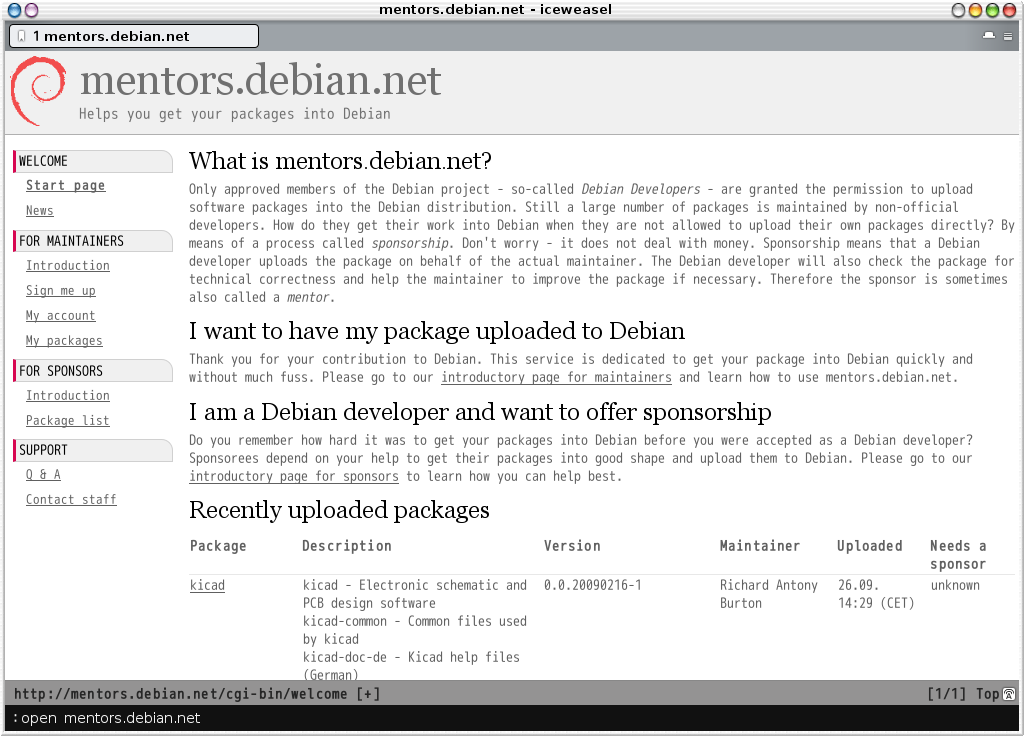
\includegraphics[scale=0.65]{image200909/mentors.png}
        \caption[mentors-top]{http://mentors.debian.net}
    \end{center}
\end{figure}

$B%5%$%H:8B&$N%a%K%e!<$K$"$k!V(BFOR MAINTAINERS$B!W$N9`L\$K$"$k(B 
$B!V(BIntroduction$B!W$r8+$F$_$F2<$5$$!#(B 
%
PM $B$,:n@.$7$?%Q%C%1!<%8$,8x<0G[I[J*$K4^$^$l$k$^$G$NN.$l$,=q$$$F$"$j$^$9!#(B
%
$B$^$?!"(B $B$3$N%Z!<%8$N2<$NJ}$K$O(B {\tt dput}$B$d(B{\tt dupload} $B$r;HMQ$7$F%=!<%9(B
$B0l<0$r(B upload $B$9$k:]$N@_DjNc$,:\$C$F$$$^$9!#(B
$BNI$/FI$s$G$*$-$^$7$g$&!#(B

$B<!$K!V(Bsign up$B!W$+$i%"%+%&%s%H$r<hF@$7$^$9!#(B
\begin{figure}[h]
    \begin{center}
        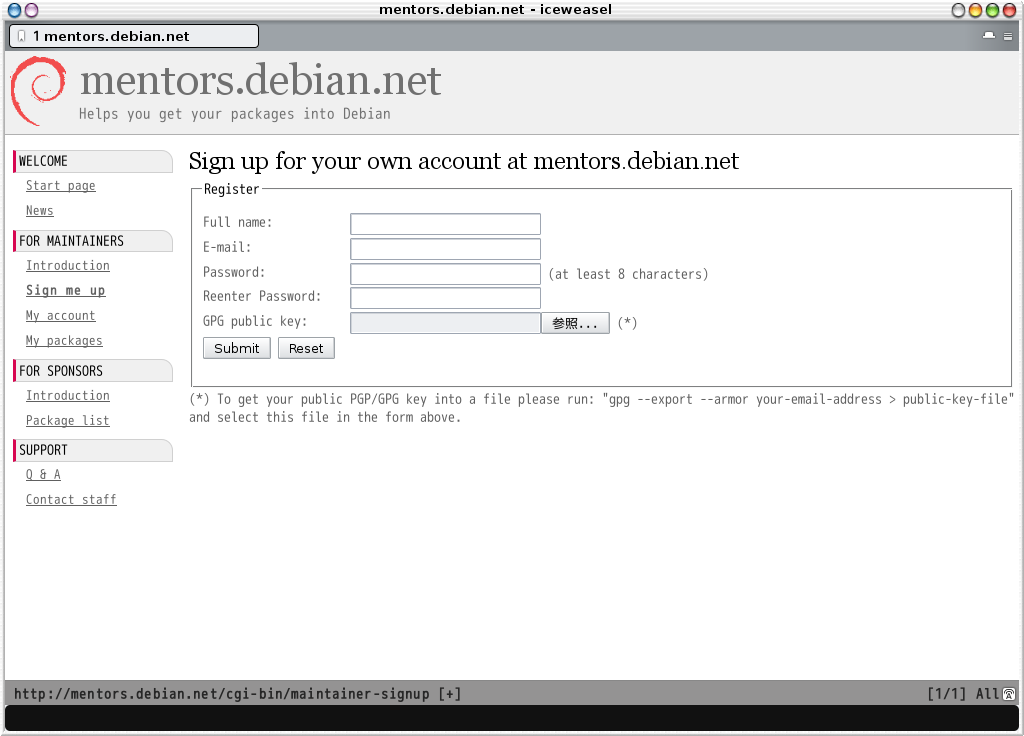
\includegraphics[scale=0.6]{image200909/mentors-signup.png}
        \caption[mentors-signup]{%
          http://mentors.debian.net/cgi-bin/maintainer-signup}
    \end{center}
\end{figure}

$B%"%+%&%s%H$N<hF@$K$O(B GPG $B8x3+80$,I,MW$K$J$j$^$9(B
$B$3$N8x3+80$O%Q%C%1!<%8:n@.;~$N=pL>$KMQ$$$?(B GPG $B80$r;HMQ$7$F2<$5$$!#(B

$B$G$O<B:]$K%"%+%&%s%H$r<hF@$7$F(B {\tt mentors.debian.net} $B$r;HMQ$7$F$_$^$7$g$&!#(B

\begin{center}
{\bf $B$*$*$C$H(B!}    
\end{center}
$B%9%]%s%5!<$rC5$9A0$K0J2<$N;v$O:Q$s$G$$$^$9$+(B?
\begin{enumerate}
      \item ITP bug report
      \item $B:n@.$9$k%Q%C%1!<%8$r(B lintian clean $B$K$9$k(B
\end{enumerate}


$B0l$DL\$O!V$3$l$+$i$3$N%=%U%H%&%'%"$N%Q%C%1!<%8$r:n@.$9$k$>(B!$B!W$H$$$&@k8@$G$9$M!#(B
WNPP -- ITP $B$H$7$F%P%0%l%]!<%H$r=q$-$^$9!#(B 
WNPP $B$O!V(BWork-Needing and Prospective Packages$B!W$NN,$G$9(B
\begin{center}
    Work-Needing and Prospective Packages: WNPP\\
    \href{http://www.debian.org/devel/wnpp}%
    {{\tt http://www.debian.org/devel/wnpp}}
\end{center}
$B%P%0%l%]!<%H=q$-J}$K$D$$$F$O(B
$B$N$,$?$5$s$NJ8>O$J$s$+$r;29M$K$7$F2<$5$$!#(B

$BFs$DL\$O%Q%C%1!<%8:n@.$N4V0c$$$N=$@5$G$9!#(B 
lintian $B$K$D$$$F$OA02s$NBg1:$5$s$NH/I=(B\cite{lintian}$B$J$s$+$r(B
$B;29M$K$7$F2<$5$$!#(B

$B$5$"=`Hw$O$G$-$^$7$?$+(B?

\subsubsection{sign up!}

$B%"%+%&%s%H<hF@$N%W%m%;%9<+BN$OHs>o$KC1=c$G$9!#(B  $BL>A0!"(B $B%a!<%k%"%I%l%9!"(B $B%Q(B
$B%9%o!<%I!"(B GPG $B8x3+80$rF~NO$7$F$7$P$7BT$A$^$7$g$&!#(B  $BEPO?$7$?%a!<%k%"%I%l(B
$B%9$K(B confirm $B%a!<%k$,Mh$^$9$N$G!"(B $B$=$3$K=q$+$l$?(B URL $B$r%V%i%&%6$G3+$$$F(B
$B2<$5$$!#(B $B%"%+%&%s%H$,M-8z$K$J$j$^$9!#(B

\subsubsection{dupload $B$N@_Dj(B}

$B%=!<%9%U%!%$%k0l<0$N%"%C%W%m!<%I$K$O(B dput $B$b$7$/$O(B dupload $B$r;HMQ$7$^$9!#(B
$B@h$:(B dupload $B%Q%C%1!<%8$rF3F~$7$^$7$g$&(B
\begin{commandline}
$ sudo aptitude install dupload
\end{commandline}
dupload $B$N@_Dj%U%!%$%k(B
$B$O(B {\tt /etc/dupload.conf} $B$b$7$/$O(B {\tt \~/.dupload.conf} $B$G$9(B.
dupload $B%Q%C%1!<%8$NDs6!$9$k(B {\tt /etc/dupload.conf} $B$K$O(B
mentors.debian.net$B$N@_Dj$,$9$G$K$"$j$^$9(B.
$B$b$7L5$$>l9g$K$O0J2<$NFbMF$r(B {\tt \~/.dupload.conf} $B$K5-=R$7$F2<$5$$!#(B
\begin{commandline}
package cofig;
$cfg{'mentors'} =
{ 
  fqdn => 'mentors.debian.net',
  incoming => '/',
  dinstall_runs => 1,
  passive => 1,
};

1;
\end{commandline}

\subsubsection{upload!}

$B$5$F!"(B $B$3$3$^$G=*$o$C$?$i(B upload $B$7$F$_$^$7$g$&(B.
$B0J2<$G$O(B rttool $B$H$$$&%Q%C%1!<%8$r(B upload $B$7$F$_$^$9(B.
\begin{commandline}
$ dupload -t mentors  rttool_1.0.3-2_amd64.changes
dupload note: no announcement will be sent.
Checking signatures before upload...GPG signature is missing
dupload fatal error: Pre-upload '/usr/share/dupload/gpg-check %1' 
failed for rttool_1.0.3-2_amd64.changes at /usr/bin/dupload line 223
\end{commandline}
...$BE\$i$l$F$7$^$$$^$7$?!#(B

$B$*E\$j$N860x$OL@3N$G$9$M!#(B $B%Q%C%1!<%8:n@.;~$K(B GPG $B=pL>$r$7$F$$$J$$$+$i$G$9!#(B
$B$3$NMM$K(B dupload $B$K$O(B {\tt .dsc} $B$d(B{\tt .changes}$B$,(B GPG $B=pL>$5$l$F$$$k$N$+!"(B
$B$J$I$N8!>Z$b9T$J$C$F$/$l$^$9!#(B

$B$G$O$A$c$s$H=pL>$7$F%Q%C%1!<%8$r:n@.$7$?8e$K:FEY(B upload $B$7$F$_$^$7$g$&!#(B
\begin{commandline}
dupload -t mentors rttool_1.0.3-2_amd64.changes
dupload note: no announcement will be sent.
Checking signatures before upload......signatures are ok
Uploading (ftp) to mentors.debian.net:/
[ job rttool_1.0.3-2_amd64 from rttool_1.0.3-2_amd64.changes
 rttool_1.0.3-2_all.deb, size ok, md5sum ok, sha1sum ok, sha256sum ok
 rttool_1.0.3-2.dsc, size ok, md5sum ok, sha1sum ok, sha256sum ok
 librt-ruby1.8_1.0.3-2_all.deb, size ok, md5sum ok, sha1sum ok, sha256sum ok
 rttool_1.0.3-2.diff.gz, size ok, md5sum ok, sha1sum ok, sha256sum ok
 rttool_1.0.3.orig.tar.gz, size ok, md5sum ok, sha1sum ok, sha256sum ok
 rttool_1.0.3-2_amd64.changes ok ]
Uploading (ftp) to mentors (mentors.debian.net)
+ FTP passive mode selected
[ Uploading job rttool_1.0.3-2_amd64
 rttool_1.0.3-2_all.deb 15.1 kB, ok (1 s, 15.07 kB/s)
 rttool_1.0.3-2.dsc 1.1 kB, ok (1 s, 1.06 kB/s)
 librt-ruby1.8_1.0.3-2_all.deb 15.2 kB, ok (2 s, 7.59 kB/s)
 rttool_1.0.3-2.diff.gz 2.7 kB, ok (1 s, 2.68 kB/s)
 rttool_1.0.3.orig.tar.gz 35.0 kB, ok (2 s, 17.48 kB/s)
 rttool_1.0.3-2_amd64.changes 1.9 kB, ok (3 s, 0.65 kB/s) ]
\end{commandline}
$BL5;v(B upload $B$5$l$?MM$G$9!#(B
$B$3$N8e!V(Bupload $B$5$l$?$h!W$H$$$&%a!<%k$,FO$-$^$9!#(B
\begin{commandline}
Subject: 'rttool' uploaded to mentors.debian.net
From: ``mentors.debian.net'' <support@mentors.debian.net>
To: uwabami@gfd-dennou.org
Date: Sat, 26 Sep 2009 16:33:47 +0200 (CEST)

Your upload of the package 'rttool' to mentors.debian.net was
successful. Sponsors can now download it. The URL of your package is:
http://mentors.debian.net/debian/pool/main/r/rttool

The respective dsc file can be found at:
http://mentors.debian.net/debian/pool/main/r/rttool/rttool_1.0.3-2.dsc
-----
\end{commandline}

{\tt mentors.debian.net} $B$K(B login $B$7$F%Q%C%1!<%8$N>pJs$r8+$F$_$^$7$g$&!#(B
\begin{figure}[h]
    \begin{center}
        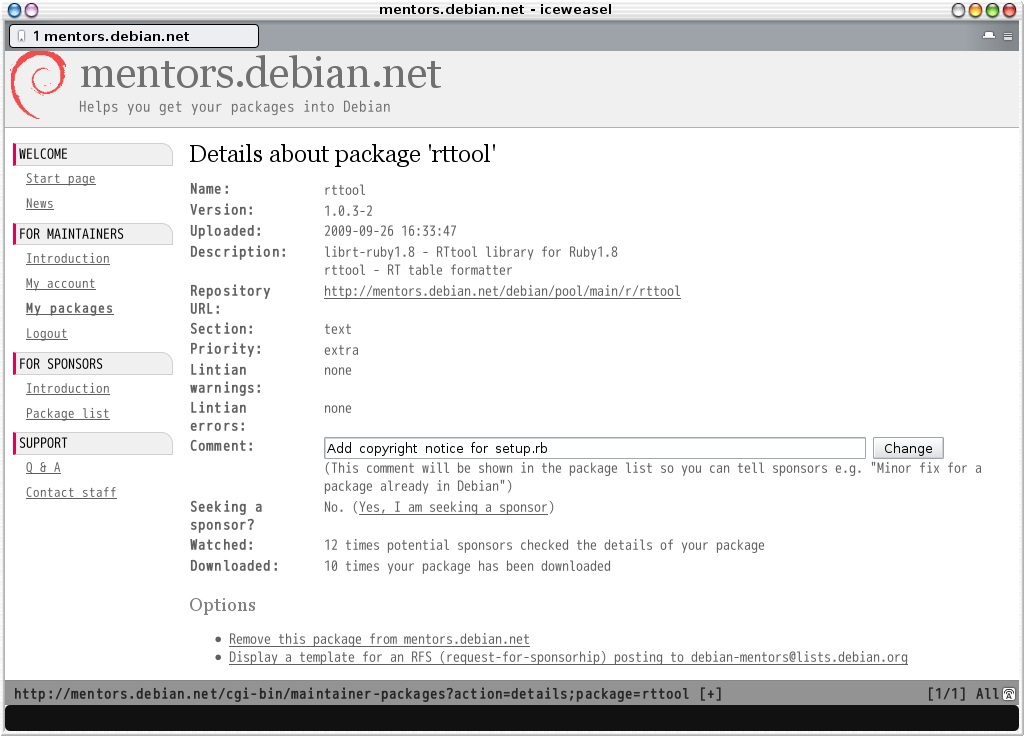
\includegraphics[scale=0.6]{image200909/mentors-package.png}
        \caption[mentors-package]{%
          http://mentors.debian.net/cgi-bin/maintainer-packages?action=details;package=rttool}
    \end{center}
\end{figure}

$B$3$N;~E@$G(B lintian warning \& error $B$,L5$$$+3NG'$7$F$*$-$^$7$g$&!#(B
unstable $B4D6-$8$c$J$$$H(B lintian $B$,8E$/$F(B check $B$7$-$l$F$$$J$$>l9g$b$"$j$^$9!#(B

$B$^$?!"(B $B%9%]%s%5!<Jg=8Cf$J$i$P!V(BSeeking a sponsor?$B!W$N9`L\$r(B $B!V(BYes$B!W(B $B$K$7(B
$B$F$*$/$HNI$$$H;W$$$^$9!#(B

$B$3$3$^$G$-$?$i=`Hw$O40N;$G$9!#(B $B%9%]%s%5!<$rJg$C$F$_$^$7$g$&!#(B
\href{mailto:debian-mentors@lists.debian.org}{{\tt debian-mentors@lists.debian.org}}$B$d(B \href{mailto:debian-devel@debian.or.jp}{{\tt debian-devel@debian.or.jp}}$B$J$I$G%9%]%s%5!<Jg=8$N%a!<%k$rAw?.$7$F$_$^$9!#(B
$B4X@>(B Debian $BJY6/2q;22C<T$G$7$?$i!"(B $BLZ2<$5$s$dBg1:$5$s$K;G$C$F$_$k$N$bNI$$$+$b$7$l$^$;$s!#(B $B4i$,$o$+$C$F$$$k?MF1;N$NJ}$,OC$,?J$_$d$9$$$+$b$7$l$^$;$s!#(B


$B!V(B\href{mailto:debian-mentors@lists.debian.org}{{\tt debian-mentors@lists.debian.org}} $B$O1Q8l$J$N$G$A$g$C$H(B...$B!W$H$$$&>l9g$b$4?4G[L5$/!#(B {\tt mentors.debian.net} $B$K(B upload $B$7$?%Q%C%1!<%8>pJs$N=j$r8+$F2<$5$$!#(B {\tt debian-mentors} $B$K%a!<%k$rAw$k$?$a$N?w7A$,$"$j$^$9!#(B $B$3$l$r85$K$7$F%a!<%k$r=q$$$F$_$k$HNI$$$G$7$g$&!#(B

\subsection{$B$^$H$a(B}

Debian $B$N(B Mentor $B@)EY$H(B {\tt mentors.debian.net} $B$K$D$$$F>R2p$7$^$7$?!#(B
$B<B:]$K$O(B mentor $B$,$_$D$+$k$+$I$&$+$ODj$+$G$O$"$j$^$;$s$N$G!"(B $BF;Dx$OD9$$$G$9!#(B

$B$^$?!"(B $B:#2s$NJ8>O$K$O(B DD $B$H$7$F%9%]%s%5!<$9$kB&$N>pJs$,$"$j$^$;$s!#(B 
Mentor $B$K$J$kB&$H$7$F!V$3$&$$$&46$8$@$H%9%]%s%5!<$K$J$j$d$9$$(B/$B$J$C$F$d$m$&$+$H$$$&5$$K$J$k!W$H$$$&$40U8+$,$"$C$?$iJ9$$$F$_$?$$!"(B $B$H;W$$$^$7$?!#(B

\begin{thebibliography}{99}
    \bibitem[1]{lintian}
  $BBg1:(B $B??!"(B 2009:
  $B!V(Blintian $B$G%Q%C%1!<%8$r%A%'%C%/$9$k!W!"(B
  $BBh(B26$B2s4X@>(B Debian$BJY6/2q(B 2009$BG/(B8$B7n(B $BG[I[;qNA(B\
  \url{http://tokyodebian.alioth.debian.org/pdf/debianmeetingresume200908-kansai.pdf}
\end{thebibliography}

%-------------------------------
\dancersection{$B:#8e$NM=Dj(B}{$B$N$,$?(B $B$8$e$s(B}

\subsection{$B<!2s$N4X@>(BDebian$BJY6/2q(B}

$B<!2s$O!"(B2009$BG/(B10$B7n(B25$BF|$KBg:eJ!Eg6hL1%;%s%?!<$G9T$&M=Dj$G$9!#(B

\subsection{$B4X@>%*!<%W%s%=!<%9(B2009}

2009$BG/(B11$B7n(B6$BF|(B($B6b(B)$B$H(B2009$BG/(B11$B7n(B7$BF|(B($BEZ(B)$B$KBg:eFn9A(BATC$B$K$F3+:E$5$l$k!V4X@>%*!<(B
$B%W%s%=!<%9(B2009$B!W$K4X@>(BDebian$BJY6/2q$b=PE8$rM=Dj$7$F$$$^$9!#(B

\begin{itemize}
 \item KOF2009$B!'4X@>%*!<%W%s%=!<%9(B2009:

\url{http://k-of.jp/2009/index.html} 

\end{itemize}


% $B:};R$K$9$k$?$a$K!"(B4$B$NG\?t$K$9$kI,MW$,$"$k!#(B
% $B$=$N$?$a$ND4@0(B
% \dancersection{$B%a%b(B}{}
% \mbox{}\newpage
% \mbox{}\newpage

\printindex
 \cleartooddpage

 \begin{minipage}[b]{0.2\hsize}
  \rotatebox{90}{\fontsize{80}{80} {\gt $B4X@>%G%S%"%sJY6/2q(B} }
 \end{minipage}
 \begin{minipage}[b]{0.8\hsize}

 \vspace*{15cm}
 \rule{\hsize}{1mm}
 \vspace{2mm}
 
\includegraphics[width=2cm]{image200502/openlogo-nd.eps}
 \noindent \Large \bf Debian $BJY6/2q;qNA(B\\ \\
 \noindent \normalfont \debmtgyear{}$BG/(B\debmtgmonth{}$B7n(B\debmtgdate{}$BF|(B \hspace{5mm}  $B=iHGBh(B1$B:~H/9T(B\\
 \noindent \normalfont $B4X@>(B Debian $BJY6/2q(B $B!JJT=8!&0u:~!&H/9T!K(B\\
 \rule{\hsize}{1mm}
 \end{minipage}

\end{document}
